\hsection{Interlude:~The Linter Ruff}%
\label{sec:listExampleForErrorsAndRuff}%
%
\gitLoadAndExecPython{lists:lists_error}{}{collections}{lists_error.py}{}%
\listingPythonAndOutput{lists:lists_error}{%
A program processing lists which exhibits some subtle errors and inefficiencies.}{}%
%
\gitExec{exec:lists:lists_error:mypy}{\programmingWithPythonCodeRepo}{.}{_scripts_/mypy.sh collections lists_error.py}%
\listingToolOutput{lists:lists_error:mypy}{%
The results of static type checking with \mypy\ of the program given in \cref{lst:lists:lists_error}.}%
%
Recently, we learned that static code analysis tools can help us to discover subtle problems in our programs.
Obviously, when dealing with more complex datastructures like lists, there are also more potential problems, more mistakes that one could make.
Let us look at the very short example program \textil{lists_error.py} in \cref{lst:lists:lists_error}.
The program consists of only two lines, \pythonil{my_list: list[str] = list([1, 2, 3])} and \pythonil{print(my_list)}.
It does not have any \emph{error} in the strict sense.
We can execute it just fine and it will produce the output \textil{[1, 2, 3]} as shown in \cref{exec:lists:lists_error}.

However, upon closer inspection, we discover some issues.
In a first step, we would apply \mypy~(as~\cref{ut:mypy}) to check for problems with the types of variables.
And indeed, \cref{exec:lists:lists_error:mypy} shows us \emph{three} errors!
We defined \pythonil{my_list} as a list of strings by using the \pgls{typeHint} \pythonil{list[str]}.
However, we then set its value to be a list of three integer numbers (hence, three errors).
This is clearly wrong.

But is this all what's wrong?
\mypy~is a tool that looks for type-related errors and \emph{only} for type-related errors.
But did we \emph{only} commit type-related errors?
Are there tools that help us to find \emph{other} errors?
\Pglspl{linter} are tools for analyzing program code to identify bugs, problems, vulnerabilities, and inconsistent code styles~\cite{J1978LACPC,RJYKK2022CULTDVM}.
As promised in the title of this section, we will also use another tool to analyze this program:~the \pgls{linter}~\ruff.

\begin{figure}%
\centering%
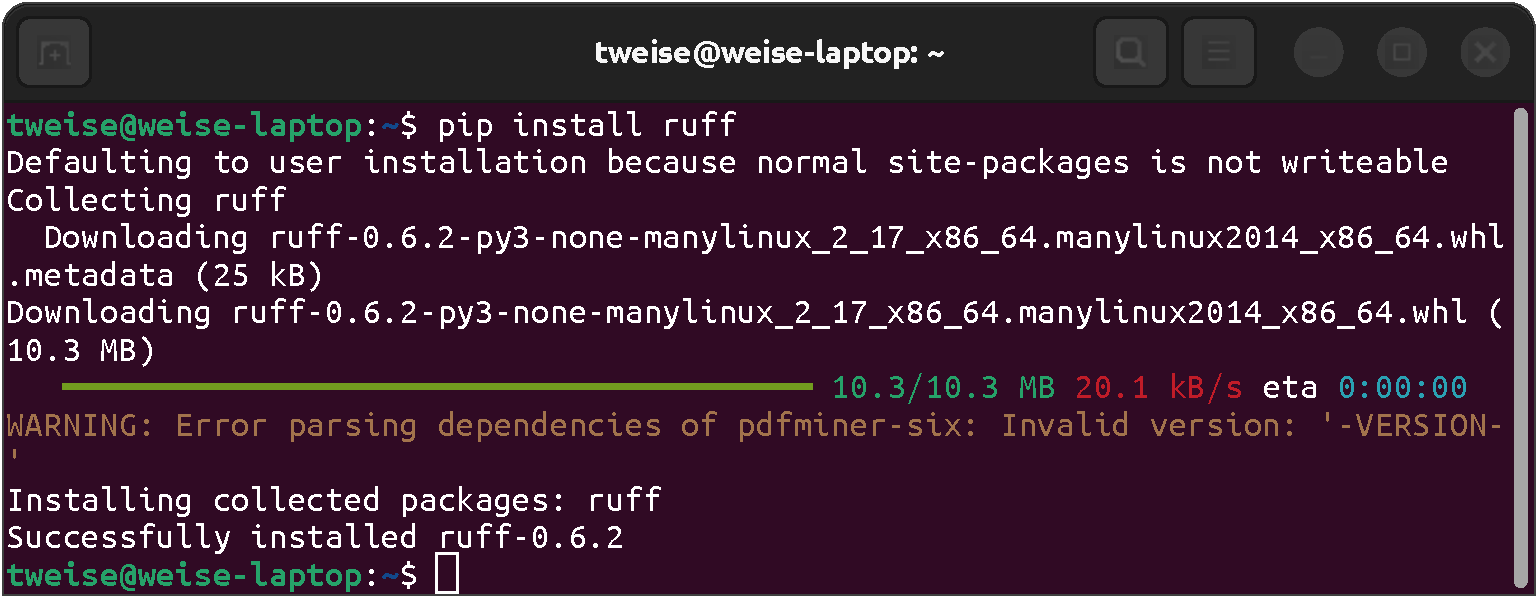
\includegraphics[width=0.7\linewidth]{\currentDir/pipInstallRuff}%
\caption{Installing \ruff\ in a \ubuntu\ \pgls{terminal} via \pip~(see \cref{sec:pipAndVenv} for a discussion of how packages can be installed).}%
\label{fig:pipInstallRuff}%
\end{figure}%
%
\usefulTool{ruff}{%
\ruff\ is a very fast \python\ \pgls{linter} that checks the code for all kinds of problems, ranging from formatting and style issues over missing documentation to performance problems and potential errors~\cite{M2022RAEFPLACFWIR}. %
It can be installed via \bashil{pip install ruff} as shown in \cref{fig:pipInstallRuff} on \cpageref{fig:pipInstallRuff}. %
You can then apply \ruff\ using the command \bashil{ruff check fileToScan.py}. %
We provide a script for using \ruff\ with a reasonable default configuration in \cref{lst:bash:ruff} on \cpageref{lst:bash:ruff}.%
}%
%
\gitExec{exec:lists:lists_error:ruff}{\programmingWithPythonCodeRepo}{.}{_scripts_/ruff.sh collections lists_error.py}%
\listingToolOutput{lists:lists_error:ruff}{%
The results of linting with \ruff\ of the program given in \cref{lst:lists:lists_error}. (We used the script given in \cref{lst:bash:ruff} on \cpageref{lst:bash:ruff} to apply \ruff.)}%
%
Let us apply \ruff\ to the program \textil{lists_error.py} given in \cref{lst:lists:lists_error}.
This can be done by executing the command \bashil{ruff check myfile.py}, where \textil{myfile.py} is the file to be checked~(you can also specify a directory).
\ruff\ has many additional parameters, which are explained at~\cite{PSF:TPPIP:R,M2022RAEFPLACFWIR}.
For example, if we want to analyze our code with respect to version~3.12 of \python, we would specify the command line argument~\textil{--target-version py312}.
With the optional \textil{--select=...} argument, we can list additional groups of rules to be checked.
As you can see, we select quite a few!
Check~\cite{M2022RAEFPLACFWIR} under \citeurl{M2022RAEFPLACFWIR} in the \emph{Rules} section for the complete list.
Sometimes, we wish to ignore some rules which do not apply to our programming scenario.
This can be done using the optional \textil{--ignore=...} argument.
You can find the complete command that we used to execute \ruff\ in the top part of \cref{exec:lists:lists_error:ruff}.
Because it is a bit long, you will probably want to create your own shell script for running \ruff\ to avoid always typing down this lengthy command.

At \ruff\ does not check for type-related errors at the time of this writing.
But -- as you can see in \cref{exec:lists:lists_error:ruff} -- it does find two other issues with our program file:
First, it complains that any python file should start with a string specifying the purpose of the file.
The use of such \pglspl{docstring} makes it easier for other programmers to understand what is done by which file in projects that are composed of multiple \python\ scripts.%
%
\bestPractice{module:docstrings}{
Each \python\ file should start with a string describing its purpose~\cite{PEP257}. %
This can either be a single line, like a headline, or a longer text. %
In the second case, the first line must be a headline, followed by an empty line, followed by the rest of the text. %
Either way, it must be a string delimited by~\pythonil{"""..."""}\pythonIdx{\textquotedbl\textquotedbl\textquotedbl\idxdots\textquotedbl\textquotedbl\textquotedbl}~\cite{PEP257,PEP8}.%
\pythonIdx{str!doc}%
}%
%
Additionally, \ruff\ finds that writing \pythonil{list([1, 2, 3])} is actually useless waste of speed and memory:
It basically creates a list as \pgls{literal} via \pythonil{[1, 2, 3]}.
Then it immediately makes a copy of it via the \pythonilIdx{list} function wrapped around the list specification.
We can leave this outer call to \pythonil{list} away.

\gitLoadAndExecPython{lists:lists_fixed}{}{collections}{lists_fixed.py}{}%
\listingPythonAndOutput{lists:lists_fixed}{%
The corrected version of~\cref{lst:lists:lists_error}, taking into account the information given by \mypy\ in \cref{exec:lists:lists_error:mypy} and \ruff\ in \cref{exec:lists:lists_error:ruff}.}{}%
%
%
In \cref{lst:lists:lists_fixed} we implement the three recommendations from the two tools.
We change the \pgls{typeHint} of the list to \pythonil{list[int]}, which solves the type confusion that \mypy\ discovered.
We remove the useless copying of the list as \ruff\ recommended.
Finally, we add a proper \pgls{docstring} at the top of the file, in which we even document the changes we applied.
The output \cref{exec:lists:lists_fixed} of the new program remains the same.
But now, both tools are satisfied, as shown in \cref{exec:lists:lists_fixed:mypy,exec:lists:lists_fixed:ruff}.
And our program is much clearer and faster.

\gitExec{exec:lists:lists_fixed:mypy}{\programmingWithPythonCodeRepo}{.}{_scripts_/mypy.sh collections lists_fixed.py}%
\listingToolOutput{lists:lists_fixed:mypy}{%
The results of static type checking with \mypy\ of the program given in \cref{lst:lists:lists_fixed}.}%
%
\gitExec{exec:lists:lists_fixed:ruff}{\programmingWithPythonCodeRepo}{.}{_scripts_/ruff.sh collections lists_fixed.py}%
\listingToolOutput{lists:lists_fixed:ruff}{%
The results of static type checking with \ruff\ of the program given in \cref{lst:lists:lists_fixed}.}

Well, this was only a two-line program.
But ask yourself:
Did you spot the incorrect \pgls{typeHint} when you read the program?
Maybe.
But did you see that we actually created a list and then copied it instead of using it directly?
(The \pgls{docstring} I give you, no chance of seeing that as we did not mention it before.)

Now imagine that your job would be to work on a program with thousands of lines that was developed by a colleague.
And remember that our program could be executed flawlessly, despite the errors.
The errors would like become problems later, though.
Wouldn't you love it if that colleague had thoroughly documented and type-hinted and checked their code?
Be that colleague.%
%
\bestPractice{manyCodeAnalysisTools}{%
Use many static code analysis tools and use them always. %
They can discover a wide variety of issues, problems, or potential improvements. %
They can help you to keep your code clean and to enforce a good programming style. %
Do not just apply them, but also \emph{implement} their suggestions wherever possible.%
}%
%
\FloatBarrier%
\endhsection%
%
